\documentclass[11pt,a4paper]{ltjsarticle}
% LuaLaTeX-ja 用の和文クラス
% コンパイルは lualatex を想定

% -------------------------------------------------
% 基本パッケージ
% -------------------------------------------------
\usepackage{amsmath,amssymb,amsthm,mathtools,bm}
\usepackage{geometry}
\geometry{margin=25mm}

\usepackage{graphicx}
\usepackage{booktabs}
\usepackage{array}
\usepackage{hyperref}
\usepackage{xcolor}
\usepackage{enumitem}
\usepackage{physics} % 好みが分かれるので不要なら外してください
\usepackage{tcolorbox}

%\usepackage{fontspec}
%\usepackage{unicode-math}

\usepackage[
    backend=biber,
    style=phys
]{biblatex}

\addbibresource{ref.bib}

\tcbuselibrary{breakable,skins,theorems}

% -------------------------------------------------
% 色設定
% -------------------------------------------------
\definecolor{myblue}{HTML}{1F4E79}
\definecolor{mygreen}{HTML}{2E7D32}
\definecolor{myred}{HTML}{B23A48}
\definecolor{myorange}{HTML}{C77700}
\definecolor{lightblue}{HTML}{EEF5FC}
\definecolor{lightgreen}{HTML}{EEF8EE}
\definecolor{lightred}{HTML}{FCEEEF}
\definecolor{lightorange}{HTML}{FFF4E5}
\definecolor{lightgray}{HTML}{F5F5F5}

% -------------------------------------------------
% ハイパーリンク設定
% -------------------------------------------------
\hypersetup{
  colorlinks=true,
  linkcolor=myblue,
  citecolor=mygreen,
  urlcolor=myred,
  pdftitle={統計力学 講義ノート},
  pdfauthor={Your Name}
}

% -------------------------------------------------
% 数式マクロ（必要に応じて追加）
% -------------------------------------------------
%\newcommand{\dd}{\mathrm{d}}
\newcommand{\ee}{\mathrm{e}}
\newcommand{\ii}{\mathrm{i}}
\newcommand{\pp}{\partial}
\newcommand{\tD}{t_\mathrm{Debye}}
%\newcommand{\Tr}{\operatorname{Tr}}
%\newcommand{\vb}[1]{\bm{#1}}

\newcommand{\avg}[1]{\left\langle #1 \right\rangle}
%\newcommand{\mc}[1]{\mathcal{#1}}

% -------------------------------------------------
% 定理環境
% -------------------------------------------------
\newtheorem{theorem}{定理}[section]
\newtheorem{proposition}[theorem]{命題}
\newtheorem{lemma}[theorem]{補題}

\theoremstyle{definition}
\newtheorem{definition}[theorem]{定義}
\newtheorem{example}[theorem]{例}

\theoremstyle{remark}
\newtheorem{remark}[theorem]{注意}

% -------------------------------------------------
% tcolorbox ベースの講義ノート用ボックス
% -------------------------------------------------

% 共通スタイル
\tcbset{
  myboxstyle/.style={
    breakable,
    enhanced,
    sharp corners,
    boxrule=0.8pt,
    left=8pt,
    right=8pt,
    top=6pt,
    bottom=6pt,
    before skip=10pt,
    after skip=10pt,
  }
}

% ポイント
\newtcolorbox{pointbox}[1][]{
  myboxstyle,
  colback=lightblue,
  colframe=myblue,
  title=ポイント,
  fonttitle=\bfseries,
  #1
}

% 注意
\newtcolorbox{cautionbox}[1][]{
  myboxstyle,
  colback=lightred,
  colframe=myred,
  title=注意,
  fonttitle=\bfseries,
  #1
}

% 直観・コメント
\newtcolorbox{intuitionbox}[1][]{
  myboxstyle,
  colback=lightgreen,
  colframe=mygreen,
  title=直観,
  fonttitle=\bfseries,
  #1
}

% 例題
\newtcolorbox{examplebox}[1][]{
  myboxstyle,
  colback=lightorange,
  colframe=myorange,
  title=例,
  fonttitle=\bfseries,
  #1
}

% 色なしの簡素な重要事項
\newtcolorbox{importantbox}[1][]{
  myboxstyle,
  colback=white,
  colframe=black,
  title=重要,
  fonttitle=\bfseries,
  #1
}

% -------------------------------------------------
% 見出しの余白調整（必要なら）
% -------------------------------------------------
\setlength{\parindent}{1em}
\setlength{\parskip}{0.3em}

% 箇条書き
\setlist[itemize]{topsep=3pt,itemsep=2pt}
\setlist[enumerate]{topsep=3pt,itemsep=2pt}

% -------------------------------------------------
% タイトル
% -------------------------------------------------
\title{くりこみ群から見たManning-Oosawa 対イオン凝集}
\author{Ryuichi Okamoto}
\date{最終更新日: \today}

\begin{document}

\maketitle
\tableofcontents


\section{はじめに}
高い線電荷密度をもつ棒状高分子電解質の周りには，実効的な線電荷密度が特定の値まで下がるだけの量の対イオンが凝集する。この現象は，Manning-Oosawa 対イオン凝集と呼ばれ\cite{Manning1969_I,Manning1969_II,Oosawa1971}，高分子電解質溶液の物理化学的性質を理解する上で重要な問題である。
このノートでは，Poisson-Boltzmann(PB)方程式を用いたManning-Oosawa 対イオン凝集の基本的な理論の解説と，その物理的描像をよりよく理解するために，PB方程式に対してKunihiro型のくりこみ群（Renormalization Group, RG）\cite{Kunihiro1995,Kunihiro1997}解析を行う。ちょっとした興味で考え始めたのだが，(論文にするようなものではないものの)少し面白くて教育的な意義もある話なので，まとめてみることにした。比較的基本的なところから説明した。必要とする知識は，電磁気学の初歩(静電場の方程式)，統計力学の初歩，微分方程式の初歩(常微分方程式)，摂動論の初歩程度である。RG解析の部分は，少しだけRGの基本的な考え方を知っていると理解しやすいと思うが，知らなくても理解できるように説明しているつもりである(そもそも筆者はRGのエキスパートではない)。

なお，このノートはもともとは筆者の個人的な，備忘録的なまとめとして書き始めたものである。また，思いついたところから10日ほどでまとめたものである。したがって内容の正確性や完全性については十分に確認できていない部分もあることをご了承いただきたい。誤りや不明点があれば，ぜひ指摘していただけるとありがたい。また，論文であれば引用すべき文献も引用していない場合があることに注意されたい。あくまで教育的なまとめであることを念頭に置いて読んでいただければ幸いである。なお，\ref{appendix:FKL}のFuoss-Katchalsky-Lifsonの厳密解の詳細に関する解説はChatGPTに書いてもらったものに筆者が若干の修正を加えたものであることを明記しておく。また，グラフを書くためのコード作成においても部分的にChatGPTにコードを書いてもらったものを筆者が確認・修正して使用している(こういう作業がAIのおかげで随分と楽になった)。


\subsection{セルモデル}
無限に長い棒状高分子電解質を考える。高分子の半径は$a$とする。\textbf{高分子は負の電荷を帯びている}とし，電荷の線密度の大きさを $\lambda(>0)$とする。この高分子は無限に長い半径$L$の円筒セルに入っているとする。円筒セルの(単位長さあたりの)体積が高分子単位長さの数密度の逆数(比容)と考えれば良い。高分子と対イオンの間にはクーロン相互作用が働き，セル内全体では電気的に中性であるとする。このようなモデルを高分子電解質のセルモデルと呼ぶ。セル内の静電ポテンシャル$\phi$はPoisson方程式
\begin{align}
\frac{1}{r}\frac{\dd}{\dd r}\left(r\frac{\dd \phi}{\dd r}\right)=-\frac{4\pi e}{\varepsilon}n(r) \label{eq:poisson}
\end{align}
を満たす。ここで$n(r)$は半径$r$の位置における対イオン(正のイオン)の数密度である。$r=a$と$L$における境界条件は，それぞれ高分子の電荷線密度と全体の電気的中性から
\begin{align}
  r\frac{\dd\phi}{\dd r}\bigg|_{r=a}=\frac{2\lambda e}{\varepsilon}, \quad r\frac{\dd\phi}{\dd r}\bigg|_{r=L}=0 \label{eq:boundary}
\end{align}
となる。



対イオンは熱平衡状態にあるとしてボルツマン分布$n(r)\propto e ^{-\beta e \phi}$を仮定($\beta=1/k_\mathrm{B}T$)すると，\eqref{eq:poisson}は$\phi$に対する非線形の方程式
\begin{align}
\frac{1}{r}\frac{\dd}{\dd r}\left(r\frac{\dd \phi}{\dd r}\right)=-\frac{4\pi e}{\varepsilon}n_0 e^{-\beta e \phi}
\end{align}
となる。これはPoisson-Boltzmann(PB)方程式と呼ばれる。ここで$n_0$は定数でポテンシャルの基準点($\phi=0$となる場所)における対イオン密度である。無次元化したポテンシャル$u=\beta e \phi$を用いると，PB方程式は
\begin{align}
  \frac{1}{r}\frac{\dd}{\dd r}\left(r\frac{\dd u}{\dd r}\right)=-4\pi \ell_Bn_0 e^{-u}, \label{eq:pb}
\end{align}
となる。ここで$\ell_B=\beta e^2/\varepsilon$はBjerrum長と呼ばれる長さのスケールで，通常の水では7\AA 程度である。境界条件\eqref{eq:boundary}は
\begin{align}
  r\frac{\dd u}{\dd r}\bigg|_{r=a}=2\xi, \quad r\frac{\dd u}{\dd r}\bigg|_{r=L}=0 \label{eq:boundary2}
\end{align}
と書き換えられる。ここで出てきた無次元パラメタ
\begin{align}
  \xi=\lambda \ell_B \label{eq:xi}
\end{align}
は\textbf{Manningパラメタ}と呼ばれ\cite{Manning1969_I,Manning1969_II}，Manning-Oosawa 対イオン凝集の重要な指標となる。あとで見るように，\textbf{PB方程式の解の振る舞いが$\xi\simeq 1$を境に大きく変わる。そして$\xi \gtrsim 1$の解と$\xi \lesssim 1$の解は，それぞれ対イオン凝集の有・無に対応}している。

\begin{pointbox}
高分子電解質溶液を，円筒状の高分子とその周りの対イオンが円筒セルに入っているモデル(セルモデル)で考える。静電場に対するPoisson方程式と対イオンが熱平衡状態にあるとの仮定からPoisson-Boltzmann(PB)方程式が導かれる。PB方程式の解の性質を決める重要な指標であるManningパラメタ$\xi=\lambda \ell_B$がPB方程式に対する境界条件から自然にあらわれる。
\end{pointbox}

\subsection{円筒形状(cylindrical geometry)の何が特別か\label{sec:cylindrical}}
Manning-Oosawa 対イオン凝集の現象は，円筒形状に由来する特別な性質に起因する。このことを見るために，PB方程式の右辺がゼロ，すなわち対イオンがない裸の荷電棒状分子を考えよう。\eqref{eq:pb}で右辺をゼロとおいた方程式が，境界条件\eqref{eq:boundary2}の一つ目(2つ目の境界条件は満たせない)のもとで
\begin{align}
  u(r)=2\xi \log(r/a) \label{eq:bare_solution}
\end{align}
が解になることは容易に確かめられる。この対数依存性は円筒形状に由来するものである。
一方で，1個の対イオンを距離$r$から$r+dr$のところにある場合の配置エントロピーを考えよう。この領域の体積は$2\pi r dr$であるから，配置の場合の数$\Omega(r)\sim 2\pi r dr$であり，配置エントロピー$S$は
\begin{align}
  S(r)\sim \log \Omega(r)\sim \log r
\end{align}
となる。つまり，対イオンの配置エントロピーも円筒形状に由来する対数依存性を持つ。したがって，円筒形状ではクーロン相互作用と配置エントロピーの両方が対数依存性を持ち，これらが競合することになる。すなわち$\xi$の大きさによって，エネルギーとエントロピーのバランスが変わることになる。このような議論はOnsagerに由来するため\cite{Onsager1934}，Manning-Oosawa対イオン凝集はOnsager-Manning-Oosawa対イオン凝集と呼ばれることもある。

一方で，球状の荷電分子の場合を考えると，対イオン配置の場合の数は$\Omega(r)\sim r^2$依存性を持つため，配置エントロピーは$S(r)\sim \log r$に比例する一方で，クーロン相互作用は$1/r$依存性を持つため，$r$が大きいところでは(球状荷電分子の電荷の多寡によらず)常にエントロピーが優勢となる。したがって，球状の荷電分子ではManning-Oosawa 対イオン凝集のような現象は起こらない。また，平面状の荷電分子の場合，荷電平面からの距離を$z$とすると，対イオン配置の場合の数は$\Omega(z)\sim dz$依存性を持つため，配置エントロピー$S(z)$は$z$依存性を持たないのに対し，クーロン相互作用は$z$に比例するため，常にエネルギーが優勢となる。したがって，対イオンは平面状の荷電分子に凝集するが，この場合はManning-Oosawa 対イオン凝集のような臨界的な現象(平面電荷密度の大小による質的変化)は起こらない。

円筒の場合に戻って，上の議論をもう少しだけ精密化してみよう。対イオン1個の分配関数$Z_1$を考える。上で述べた裸の荷電円筒に対する$u$を用いると，
\begin{align}
  Z_1
  &\sim \int_a^L dr\, 2\pi r e^{-u(r)}
  = \int_a^L dr\, 2\pi r e^{-2\xi \log(r/a)}
  \sim \int_a^L dr\, r^{1-2\xi}
\end{align}
となる。したがって$Z_1$は$\xi<1$のときは$L\to\infty$で発散(自由エネルギーは負に発散)する。この発散の原因は，対イオンが無限遠へ逃げることによるエントロピーの(無限の)増加である。一方，$\xi>1$のときは発散しない。これは$\xi>1$のときには対イオンが無限遠に逃げても有限のエントロピーしか得られないことを意味する。したがって，対イオンが高分子に強く束縛されて，あるいは凝集して実効的な(くりこまれた)Manningパラメタ$\xi_R$を小さくすることで自由エネルギーを下げることができる。$\xi_R>1$である限り，凝集することで自由エネルギーを下げられるので，結局$\xi_R$は1にまで下がることになる。逆に，$\xi_R$が１を下回ってしまうと仮定すると，対イオンが無限遠に逃げることで自由エネルギーを下げられることになるので，$\xi_R$は1にまで上がることになる。したがって，$\xi>1$のときには対イオンが高分子に凝集して実効的な$\xi_R$が1になるような状態が安定になることになる。これがManning-Oosawa 対イオン凝集の物理的な描像である。

この現象は，PB方程式を解くことでより精密に議論できる。Manning-Oosawaの対イオン凝集は，PB方程式の解の性質が$\xi$が1を境に大きく変わることに対応する。より正確にいうと，上の議論で$L$が無限大(現実系に対応させれば高分子濃度が無限小)で議論をしたことからも推測されるように，PBの解が大きく変わる$\xi$は$L$が有限の場合は1からずれる。また，PB解の変化も無限希釈極限$L\to\infty$で特に顕著になる。その意味では\textbf{Manning-Oosawa 対イオン凝集を一種の転移と見ることができるのは無限希釈極限$L\to\infty$においてである。}

\section{Fuoss-Katchalsky-Lifsonの厳密解}
実は，PB方程式\eqref{eq:pb}, \eqref{eq:boundary2}には厳密解が知られている。Fuoss-Katchalsky-Lifsonの厳密解と呼ばれるものである\cite{Fuoss1951}。これを紹介しておく。
まず，対数座標
\begin{equation}
t=\log(r/\ell_B)
\end{equation}
を導入する。対数座標では，スケール変換$r\to \lambda r$が$t\to t+ \log\lambda$のように並進になる。この座標ではPB方程式\eqref{eq:pb}は
\begin{align}
  \frac{d^2 u}{dt^2} = -4\pi n_0\ell_B^3 e^{-u+2t}, \label{eq:pb_t}
\end{align}
と書ける。
境界条件\eqref{eq:boundary2}は
\begin{align}
  \frac{du}{dt}\bigg|_{t=t_a}=2\xi, \quad \frac{du}{dt}\bigg|_{t=t_L}=0 \label{eq:boundary_t}
\end{align}
となる。ただし，$t_a=\log(a/\ell_B)$, $t_L=\log(L/\ell_B)$である。
詳細は\ref{appendix:FKL}に記したが，この厳密解は$\xi$, $L$, $a$をパラメタにもつ超越方程式から決定される無次元数$\gamma$を用いて表される。この解は$\xi$がある臨界値$\xi_c$を境に，三角関数型の解と双曲線関数型の解に分かれる。$\xi>\xi_c$のときには三角関数型の解が現れるが，$\xi<\xi_c$のときには双曲線関数型の解が現れる。$\xi=\xi_c$のときには有理関数型の解が現れる。この臨界値は
\begin{align}
  \xi_c = \frac{\log(L/a)}{1+\log(L/a)}
\end{align}
で与えられ，特に$L/a\to\infty$の無限希釈極限では$\xi_c$は1に近づく。
\begin{figure}[htbp]
  \begin{center}
    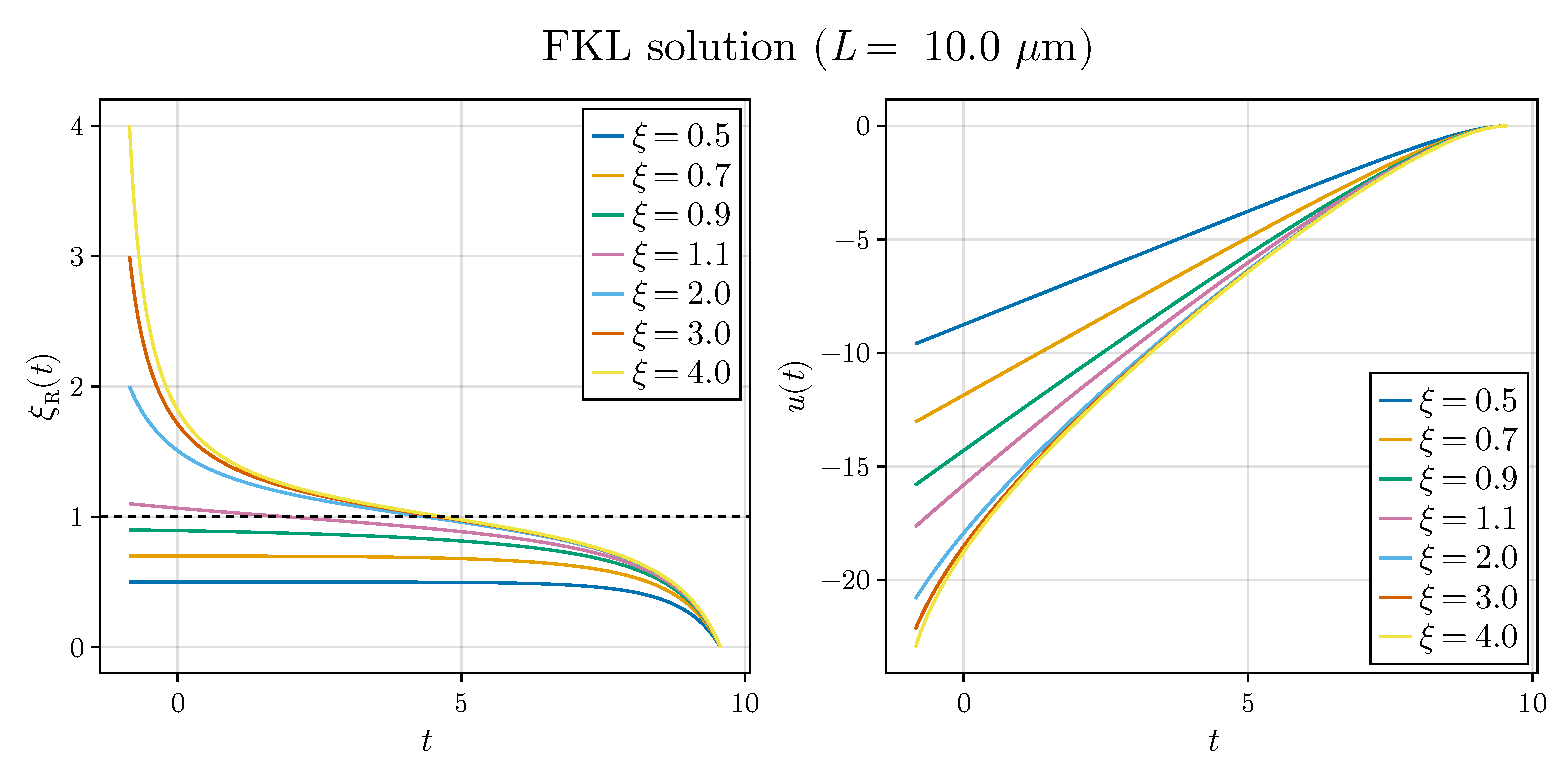
\includegraphics[width=0.8\textwidth]{./code/katchalsky10.0}
    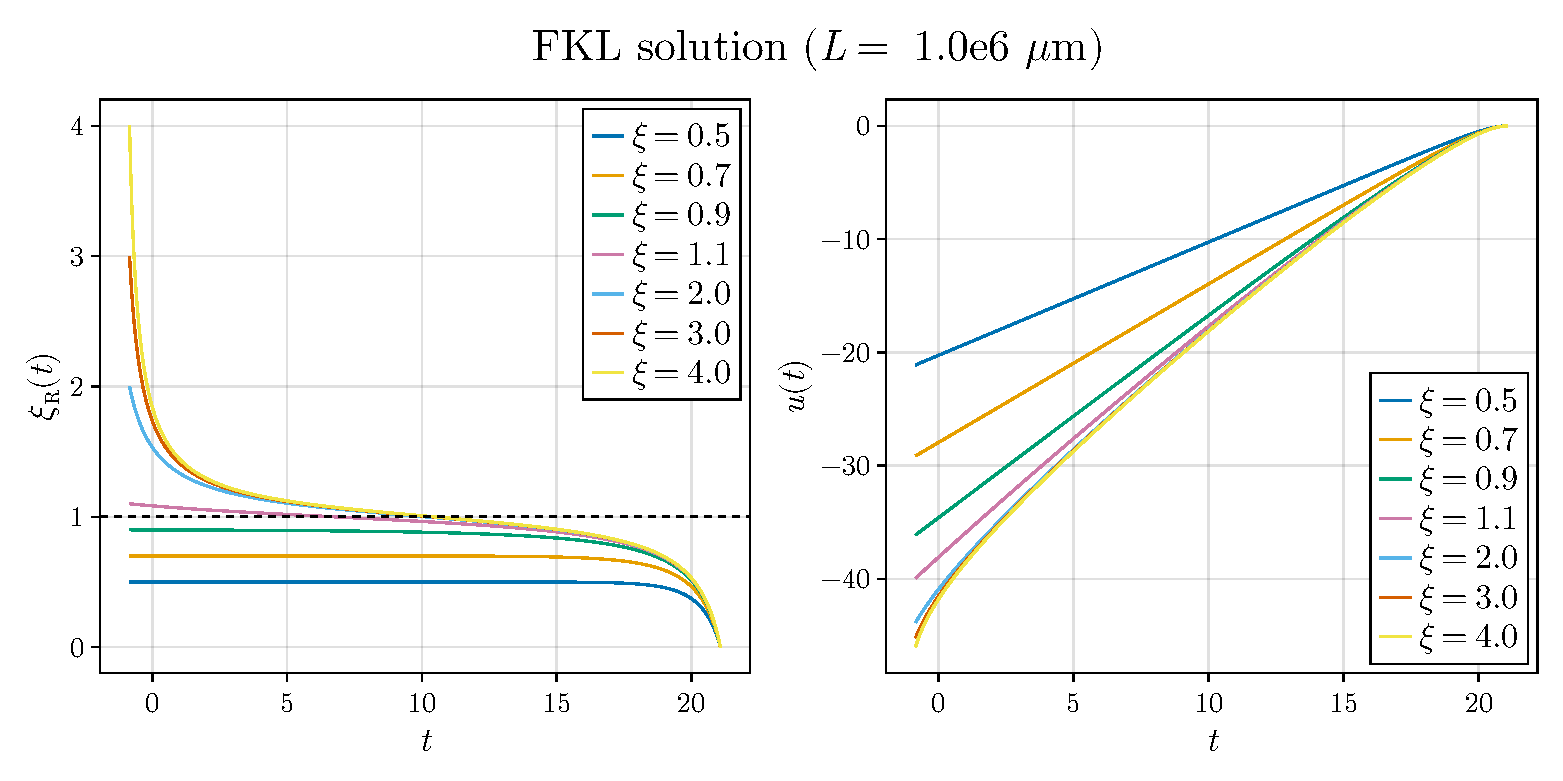
\includegraphics[width=0.8\textwidth]{./code/katchalsky1.0e6}
    \caption{Fuoss-Katchalsky-Lifsonの厳密解の例。左側にくりこまれたManningパラメタ$\xi_R(t)$，右側にポテンシャル$u(t)$を示した。$\ell_B=7$ \AA , $a=3$ \AA とした。上の図では$L=10 \mu$m, 下では$L=10^6 \mu$mとした。\label{fig:FKL}}
  \end{center}
\end{figure}

解の特徴を見るために，各$t$におけるくりこまれた(renormalized) Manningパラメタ(あるいは電荷線密度)$\xi_R(t)$を
\begin{align}
  \xi_R(t) \equiv \frac{1}{2}\frac{du(t)}{dt}
\end{align}
と定義する。これは，単位長さあたりの棒の電荷数と，$t_a$から$t$までにある対イオンの数を足し合わせたものである。したがって，棒の電荷が対イオンによって部分的に遮蔽された有効電荷密度とも言える。



図\ref{fig:FKL}にFKLの厳密解の例を示した。左側にくりこまれたManningパラメタ$\xi_R(t)$，右側にポテンシャル$u(t)$を示した。$\ell_B=7$ \AA , $a=3$ \AA とした。上段では$L=10 \mu$m, 下段では$L=10^6 \mu$m，したがってそれぞれの臨界値は$\xi_c\simeq0.91$と$0.96$である。まず，$\xi<\xi_c$の例(0.5, 0.7, 0.9)では，広い$t$の領域で$\xi_R(t)\simeq\xi$となっていることがわかる($t=t_L$では境界条件$\xi_R(t_L)=0$を課していることに注意)。これは対イオンが高分子近傍に凝集していない(広がろうとするエントロピー効果が優勢)ことを示している。一方，$\xi>\xi_c$の例(1.1, 2, 3, 4)では，$\xi_R(t)$は$t$が大きくなるとともに減少している。特に注目すべきは，$\xi=2$, 3, 4の$\xi_R(t)$が$t\gtrsim 4$ではほぼ重なることである。対応して，$u(t)$も重なる。すなわち，$\gtrsim 4$だけを観察する限りにおいては，これら三つの高分子の電荷密度の見分けがつかないことを意味する。このような振る舞いは$L$が大きい(高分子が希薄)ほど顕著になる。実際，$L=10^6\mu$mの場合は$\xi=1.1$の曲線も$10\gtrsim t$でほぼ重なることがみてとれる。\textbf{無限希釈極限($L\to\infty$)では$\xi_c\to1$となり，$\xi>1$のあらゆる$\xi$に対して，高分子近傍を除く$t$の広い領域で$\xi_R(t)$が同一曲線に乗ることになる。反対に$\xi<1$では$t$の広い領域でほぼ一定値$\xi_R(t)\simeq \xi$となる。} これがManning-Oosawa 対イオン凝集・非凝縮の特徴である。

\begin{pointbox}[title=重要(FKLの厳密解の特徴)]
Manningパラメタ$\xi$が臨界値$\xi_c(\approx 1)$より大きい場合，高分子近傍を除く領域で$\xi_R(t)$や$u(t)$が同一曲線に乗る。これは高分子近傍から離れれば，高分子の電荷量がいくらか見分けがつかない($\xi\approx 1$と見分けがつかない)ことを意味する。逆に$\xi<\xi_c$では，高分子から遠方$t\sim t_L$を除く広い範囲で$\xi_R(t)\simeq \xi$となる。高分子が希薄(セルサイズ$L$が大)では特にこれらの振る舞いは顕著になり，$\xi_c$はより1に近づく。無限希釈($L\to\infty$)では$\xi_c\to 1$となる。
\end{pointbox}

\section{RG解析}
前節で見たように，PB方程式の厳密解はManningパラメタ$\xi$が臨界値$\xi_c$をまたぐ時に質的に変化する。$\xi>\xi_c$の解がManning-Oosawa凝集に対応し，$\xi<\xi_c$が非凝集に対応することは既に説明したとおりである。\ref{appendix:FKL}にあるように，FKLの厳密解は，\textbf{その式をみるだけで簡単に振る舞いが即座に見えるというものではなく，特に無次元数$\gamma$を決定する超越方程式の振る舞いを分析する必要がある}。これによってManning-Oosawa凝集現象を式で理解することも可能ではある。

しかし，ここではあえて，その代わりにPB方程式に対してKunihiro型のくりこみ群(Renormalization Group, RG)解析を行うことで，Manning-Oosawa凝集現象をより直観的に理解することを試みる。くりこみ群は，もともと場の量子論や統計力学における臨界現象の解析において，エネルギースケール（あるいは長さスケール）の変化に伴う実効的な相互作用の変化を記述する方法として発展した。一方，Oono，Chen，Goldenfeldらは，場の理論におけるくりこみ群と類似の考え方を用いて，非線形微分方程式の漸近解を系統的に構成する方法を提案した\cite{ChenGoldenfeldOono1994,GoldenfeldOono1996}。その後 Kunihiro により，Oonoらの方法は，\textbf{各点で与えられた局所的に精度の良い解の族の包絡線を構成することで，大域的に一様に有効な近似解を構成する方法}として再定式化された\cite{Kunihiro1995,Kunihiro1997}。本稿では，この方法を Kunihiro 型のRG解析と呼ぶ。

PB方程式にはFKLの厳密解が存在するため，あえて近似的なRG解析をする必要は無いと言えばそのとおりであるが，これから見るようにRG解析は，PB方程式の解の振る舞いをより直観的に理解するために有用である。特に，$\xi$が臨界値$\xi_c$をまたぐときに解の振る舞いが大きく変わることを，RG解析の観点から理解することができる。さらに，RG解析はFKLの厳密解では直接的には見えにくいPB方程式の解の構造を明らかにすることもできる。例えば，$\xi>\xi_c$のときのPB方程式の解が$t$の広い領域で同一曲線に乗ることは前述した。RG解析ではこの現象を後述の$\beta$関数の振る舞いから，より簡単に理解することができる。

方針は以下の通りである。まず，各$t_a<t_R<t_L$に対してPB方程式の``局所的に良い解"の族を構成する。ここで，$t_R$は解の族のパラメタとなる。次に，この解の族の包絡線を構成することで，PB方程式の大域的に有効な近似解を構成する。包絡線を構成する方程式はRG方程式と呼ばれる。この方程式は，全ての$t$に対して$t_R$に依らずに同一の解を与えることを要求する方程式になっており，RG方程式と呼ばれる所以である。RG方程式は，PB方程式の解の族の``境界条件"である$\xi_R$の$t$に対する微分方程式となる。RG方程式の$\beta$関数(後述)の振る舞いを見ることで，PB方程式の解の振る舞いを理解することができる。
\subsection{計算}
まず$v=du/dt$とおいて，PB方程式\eqref{eq:pb_t}を以下のように書き換える。
\begin{align}
  \frac{dv}{dt} = -4\pi C \epsilon e^{-u+2t}, \quad \frac{du}{dt} = v \label{eq:pb_first_order}
\end{align}
ここで，$C=n_0\ell_B^3$，そして$\epsilon >0$はbookkeeping パラメタで，このパラメタが微小であるとして摂動計算した後で$\epsilon=1$とする。まず，$t_a<t_R<t_L$を満たす任意の$t_R$に対して，境界条件
\begin{align}
  v(t_R) = 2\xi_R(t_R), \quad v(t_L) = 0 \label{eq:boundary_tR}
\end{align}
を満たすPB方程式の解を近似的に構成する。そこで，$v=v_0+\epsilon v_1 + \cdots$，$u=u_0+\epsilon u_1 + \cdots$と展開する。$O(\epsilon^0)$の方程式は
\begin{align}
  \frac{dv_0}{dt} = 0, \quad \frac{du_0}{dt} = v_0 \label{eq:pb_order0}
\end{align}
である。これは簡単に解けて，
\begin{align}
  v_0(t) = 2\xi_R, \quad u_0(t) = 2(t-t_R)\xi_R  + u_{0R} \label{eq:pb_order0_solution}
\end{align}
となる。ここで，境界条件は\eqref{eq:boundary_tR}の一つ目だけを使った。式\eqref{eq:pb_order0_solution}の$u_0$は裸荷電円筒によるポテンシャル($\sim \log r$)になっていることに注意。これが以下に見るように摂動1次解が$\xi_R=1$で振る舞いが変わることの鍵となっている。 1次摂動$O(\epsilon^1)$の方程式は
\begin{align}
  \frac{dv_1}{dt} = -4\pi C e^{-u_0+2t}, \quad \frac{du_1}{dt} = v_1 \label{eq:pb_order1}
\end{align}
である。これから$v_1$の解は
\begin{align}
  v_1(t) = -4\pi C \int_{t_R}^t dt' e^{-u_0(t')+2t'}=\frac{4\pi Ce^{-u_{0R}+2t_R}}{2(\xi_R-1)} \left[ e^{-2(\xi_R-1)(t-t_R)}-1\right] \label{eq:v1_solution}
\end{align}
と求まる。したがって$\epsilon$の1次の近似解は($\epsilon=1$とおいて)
\begin{align}
  v(t;t_R) = 2\xi_R + \frac{4\pi Ce^{-u_{0R}+2t_R}}{2(\xi_R-1)} \left[ e^{-2(\xi_R-1)(t-t_R)}-1\right] \label{eq:v_approx}
\end{align}
となる。ここで境界条件\eqref{eq:boundary_tR}の二つ目を使うと，
\begin{align}
  4\pi C e^{-u_{0R}+2t_R} = \frac{4\xi_R(\xi_R-1)}{1-e^{-2(\xi_R-1)(t_L-t_R)}} \label{eq:u0R_solution}
\end{align}
であるから，これを\eqref{eq:v_approx}に代入して，
\begin{align}
  v(t;t_R) = 2\xi_R + \frac{2\xi_R}{1-e^{-2(\xi_R-1)(t_L-t_R)}} \left[ e^{-2(\xi_R-1)(t-t_R)}-1\right] \label{eq:v_approx_final}
\end{align}
となる。これが$t_R$をパラメタとするPB方程式の解の族である。任意の$t_R$についてこの解の族が同一の$v(t)$を与えることを要請する。すなわち，
\begin{align}
  0=\left.\frac{\partial v(t;t_R)}{\partial t_R}\right|_{t_R=t} \label{eq:RGE}
\end{align}
である。これがRG方程式であり，\textbf{くりこまれたManningパラメタ$\xi_R(t)$に対する微分方程式を与える}。このRG方程式の解$\xi_R(t)$を式\eqref{eq:v_approx_final}に代入し$t_R=tとすることで$，元のPB方程式の大域的に有効な近似解$v(t)\simeq 2\xi_R(t)$が得られる。RG方程式についてKunihiroは以下の洞察を得た: (i)式\eqref{eq:RGE}で微分の後に$t_R=t$とおいた理由は，$t_R$の解は$t$に近づくほど(摂動項の寄与が小さくなるから)精度が上がると考えられるからである。(ii)式\eqref{eq:RGE}は数学的には$t_R$をパラメタとするPB方程式の解の族の($t$で接する)包絡線を構成する方程式になっている。これら二つの洞察は，RGが局所的に精度の良い解の族の包絡線を構成することで大域的に有効な近似解を構成する方法であることを示している。ただし，今回の例では以下の点に注意が必要である。
\begin{cautionbox}[title=やや進んだ注釈]
普通のRG解析では，$\epsilon (t-t_R)$ のような形の永年項（secular term）が現れるように摂動展開を組むことが多い。そしてRGは，このような永年項の累積効果をくりこまれた係数に吸収することで，解の大域的振る舞いを記述する。ところが今回は式\eqref{eq:v_approx_final}のように，$t-t_R$ が指数関数の中に入った形の項が現れる。このような項は，通常の $\epsilon (t-t_R)$ 型の永年項とは異なり，一般には relevant な方向に対応し，その効果を単純な slow variable の流れとして記述することは難しい。

しかし今回の解析では，摂動解の構成において $t=t_R$ だけでなく $t=t_L$ での境界条件も用いており，局所解の族には局所的な情報だけでなく大域的な情報もあらかじめ組み込まれている。その意味で，本解析は，局所解の包絡線を構成することで大域的に一様な近似解を得るという標準的な Kunihiro 型RG解析とはやや異なる性格を持っている。したがって，本解析では式\eqref{eq:v_approx_final}のような形の項が現れる場合でも，有効的なRG方程式を構成することができたと思われる。

もう少し細かいことを述べると，Kunihiro型のRGは，(i)解の初期値(境界値)を定める場所$t_0$とその値$v(t_0),u(t_0)$に解そのものが依存しない，というWilson RG的な原理の部分と，(ii)その摂動実装としての永年項の出現や包絡線, slow variable選択とslave variable調整といった詳細の二重構造になっているととらえられる。今回の解析では，(i)のWilson的原理はそのまま保持している。一方で (ii) については，通常の Kunihiro 型RGのように
$t=t_0$ 近傍の情報だけから局所解を構成するのではなく，外側境界 $t=t_L$ における条件も用いて局所解族を構成している。したがって，本解析でも包絡線構成そのものは行われているが，包絡線を構成する局所解はあらかじめ大域的情報を含んでいる。この意味で，本解析は通常の初期値問題に対するKunihiro 型RGと，Wilson 的な running coupling の構成との中間的な性格を持つものと解釈することができる。

ちなみに，今回は $4\pi C e^{-u+2t_R}$ という項全体を摂動として扱いRG方程式を構成したが，代わりに $4\pi C e^{-\epsilon u+2t_R}$ のように指数を$\epsilon$で展開してRG方程式を構成することも可能である。この場合には $\epsilon (t-t_R)$ 型の永年項が現れ，より標準的なRG解析に近い形となる。しかしこの場合にはRG方程式の $\beta$ 関数の構造が変化し，$\xi$ が臨界値をまたいだ際の特徴的な振る舞いは弱くなる。このやり方では非線形性を弱め過ぎていて，Manning--Oosawa凝集の本質的な非線形効果を十分に記述できなくなるためと考えられる。一方，本解析では非摂動解として裸の荷電円筒の解($\sim \log r$)を採用し，かつ対イオンエントロピー($\sim \log n(r)$)の直接的帰結である$e^{-u}$の項をそのままの形で摂動として入れているため，\ref{sec:cylindrical}節で議論したエネルギーとエントロピーの拮抗が自然に取り込まれていると考えられる。RGの観点からは，非線形項 $e^{-u}$をそのまま保持することで，裸の円筒ポテンシャルと対イオンエントロピーの競合に由来するスケーリング構造が保存されていると解釈できる。
\end{cautionbox}

\subsection{$\beta$関数の振る舞いとManning-Oosawa凝集}
さて，式\eqref{eq:RGE}を具体的に書き下すと，
\begin{align}
  \frac{d\xi_R}{dt} = \beta(\xi_R;t_L,t) \equiv -\frac{2\xi_R(\xi_R-1)}{1-e^{-2(\xi_R-1)(t_L-t)}} \label{eq:beta_function}
\end{align}
となる。この$\beta$関数の振る舞いを調べることで，PB方程式の解の振る舞いを理解することができる。まず，$\beta <0$であり，したがって$\xi_R$は$t$とともに減少する。このことは，$t$ (したがって$r$)が増加するにしたがって内側に含まれる対イオンの数が増えていくので物理的に当然の結果である。また，$t\simeq t_L$では，$\beta \simeq -2\xi_R/(t_L-t)$となる。したがって，$t$が$t_L$に近づくにつれて$\xi_R\sim (t_L-t)^2$のように減少して0に近づくことになる。このことは，PB方程式の境界条件$\xi_R(t_L)=0$とくりこみ群の流れが整合することを示している。以下では$t_L\gg 1$，つまり高分子が十分希薄であることを仮定する。このとき以下のことがわかる:
\begin{itemize}
  \item 高分子近傍，すなわち$t_L - t\gg1$で，$\xi_R$が1よりある程度大きい場合，分母の指数関数は無視できて，$\beta \simeq 2\xi_R(\xi_R-1)$となる。このとき$\log(\xi_R/(\xi_R-1))\sim 2t$であるから$\xi_R$が$t$とともに減少することがわかる。したがって$\xi_R\gg 1$のときには$\xi_R\sim t^{-1}$で減少し，$\xi_R$が1に近づくにつれて$\xi_R-1\sim e^{-2t}$で1に近づくことがわかる。この振る舞いは$t_L$が大きい(高分子が希薄)ほど顕著になる。
  \item $t_L-t$を有限に保って$\xi_R$が1の極限を考える。このとき分母$\sim 2(\xi_R-1)(t_L-t)$となるので，$\beta \to -2/(t_L-t)$となる。したがって，高分子近傍で$t_L-t$が十分大きいときには$\xi_R$は1のままほとんど変化しない。特に高分子希薄極限では$\xi_R$はひとたび1に達するとその後は``流れない''ことになる。
  \item $\xi_R$が1よりある程度小さい場合，つまり，$2(1-\xi_R) \gg (t_L-t)^{-1}$のとき，$\beta \simeq 2\xi_R(\xi_R-1)e^{-2(1-\xi_R)(t_L-t)}$となる。したがって，$|\beta|$は非常に小さくなり，$\xi_R$はほとんど変化しない。この結果と１つ前の結果を合わせると，\textbf{高分子近傍では，$\xi_R\lesssim 1$のときには$\xi_R$はほとんど変化しない}ことになる。
\end{itemize}

\begin{figure}[htbp]
  \begin{center}
    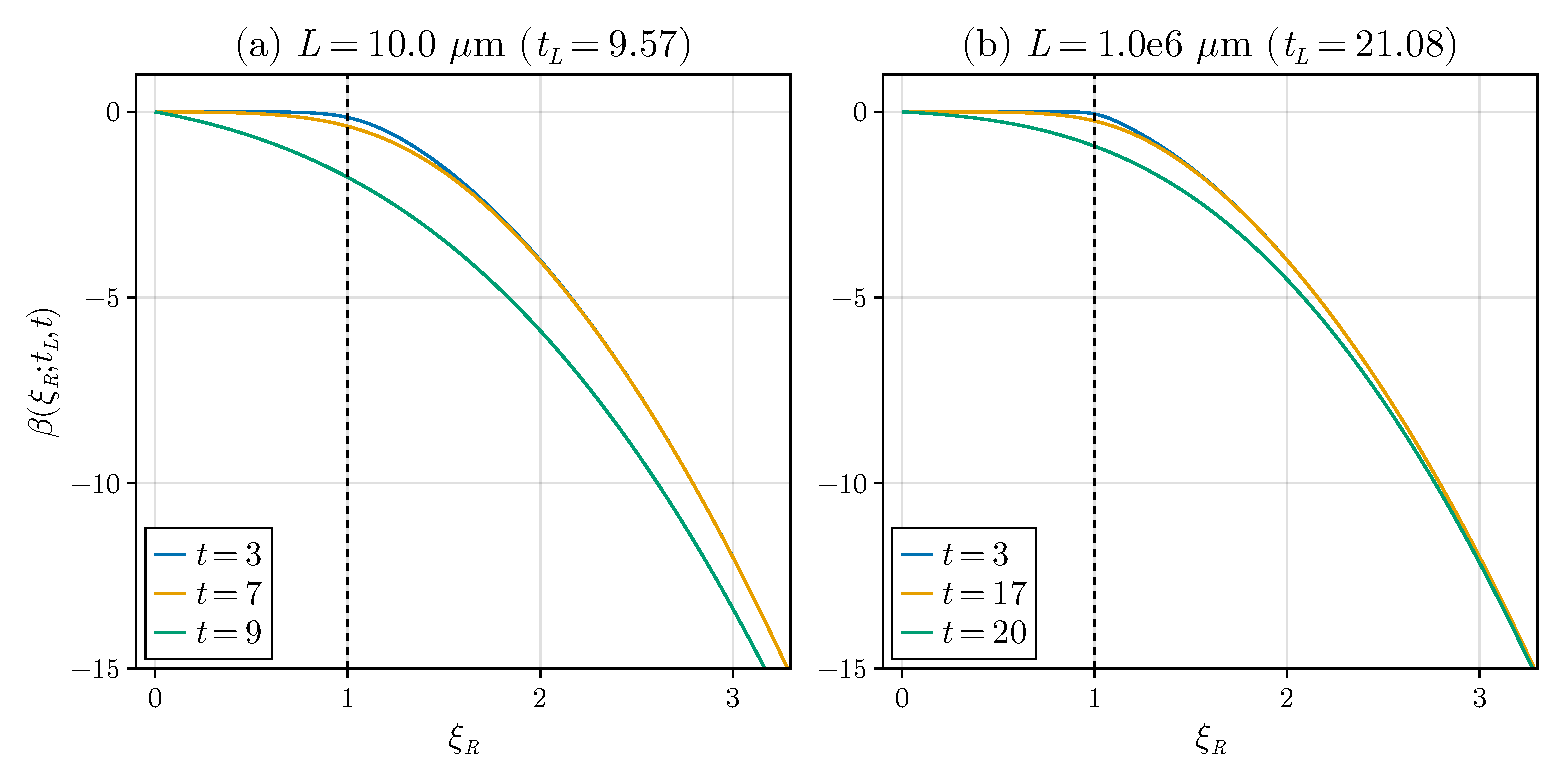
\includegraphics[width=0.9\textwidth]{./code/beta}
    \caption{$\beta$関数の振る舞い。(a) $L=10 \mu$m ($t_L=9.57$)とし，$t=3,7,9$とした。 (b) $L=10^6 \mu$m ($t_L=21.08$)とし，$t=3,17,20$とした。\label{fig:beta}}
  \end{center}
\end{figure}
図\ref{fig:beta}には$\beta$関数をプロットした。(a)$L=10 \mu$m ($t_L=9.57$)，$t=3,7,9$とした場合と，(b) $L=10^6 \mu$m ($t_L=21.08$)，$t=3,17,20$とした場合である。これらの図からも上に述べた性質が見て取れる。まず，$t$が$t_L$に近いときには$\beta$は$\xi_R$の全領域で有限となり，$t$が$t_L$に近づくにつれて$\xi_R\to 0$，すなわち境界条件と整合する。 重要なのは，$t$が$t_L$にそれほど近く無い場合には，$\xi_R\gtrsim 1$のときには$\beta$は有限で，$\xi_R$が1に近づくにつれて0に近づいていくことである。また，$\xi_R\lesssim 1$のときには$|\beta|$は非常に小さくなり，$\xi_R$がほとんど変化しないこともわかる。特に高分子が希薄な場合(b)には，この振る舞いが顕著になる。すなわち，$\xi=\xi_R(t_a)$が1より大きいときには，$\xi_R$は$t$とともに減少していくが，$\xi_R$が1に近づくにつれて$\beta$が0に近づいていくため，$\xi_R$は1のままほとんど変化しないことになる。すなわち，\textbf{$\xi>1$の解は全て$t$が大きくなるにつれて同一曲線($\xi=1$の場合の解)に乗る。逆に$\xi=\xi_R(t_a)$が1より小さいときには，$\xi_R$は$\xi$のままほとんど変化しない}ことになる。これらの振る舞いは，FKL解で見た解の振る舞いと(少なくとも定性的には)同じであり，Manning-Oosawa凝集・非凝集現象そのものである。

このように，RG方程式に現れる$\beta$関数の振る舞いを調べることで，Manning-Oosawa凝集現象を容易に理解することができる。特に，FKLの厳密解の式は複雑で一見して解の振る舞いが理解できないのに対して，$\beta$関数は比較的単純な式であり，その振る舞いが容易に理解できる。

\subsection{RG方程式の数値解}
ここまでに見たように，$\beta$関数の振る舞いからPB方程式の解の振る舞いが理解できる。ここでは確認のため，実際にRG方程式\eqref{eq:beta_function}を数値的に解いてみる。図\ref{fig:RG}では様々な初期条件$\xi_R(t_a)=\xi$に対して，数値的に式\eqref{eq:beta_function}を積分した結果をプロットした。パラメタは図\ref{fig:FKL}と同じである。Manningパラメタ$\xi$が1より大きい時は$t$が大きくなるにつれて$\xi_R$は速やかに減少し，同一曲線に乗る。一方$\xi<1$のときは$t_L$近傍を除けば$\xi_R\simeq \xi$となっている。セルサイズ$L$が大きいほうがこのような特徴が顕著である。これらは図\ref{fig:FKL}でみたFKL厳密解の振る舞いと同じである。

\begin{figure}[htbp]
  \begin{center}
    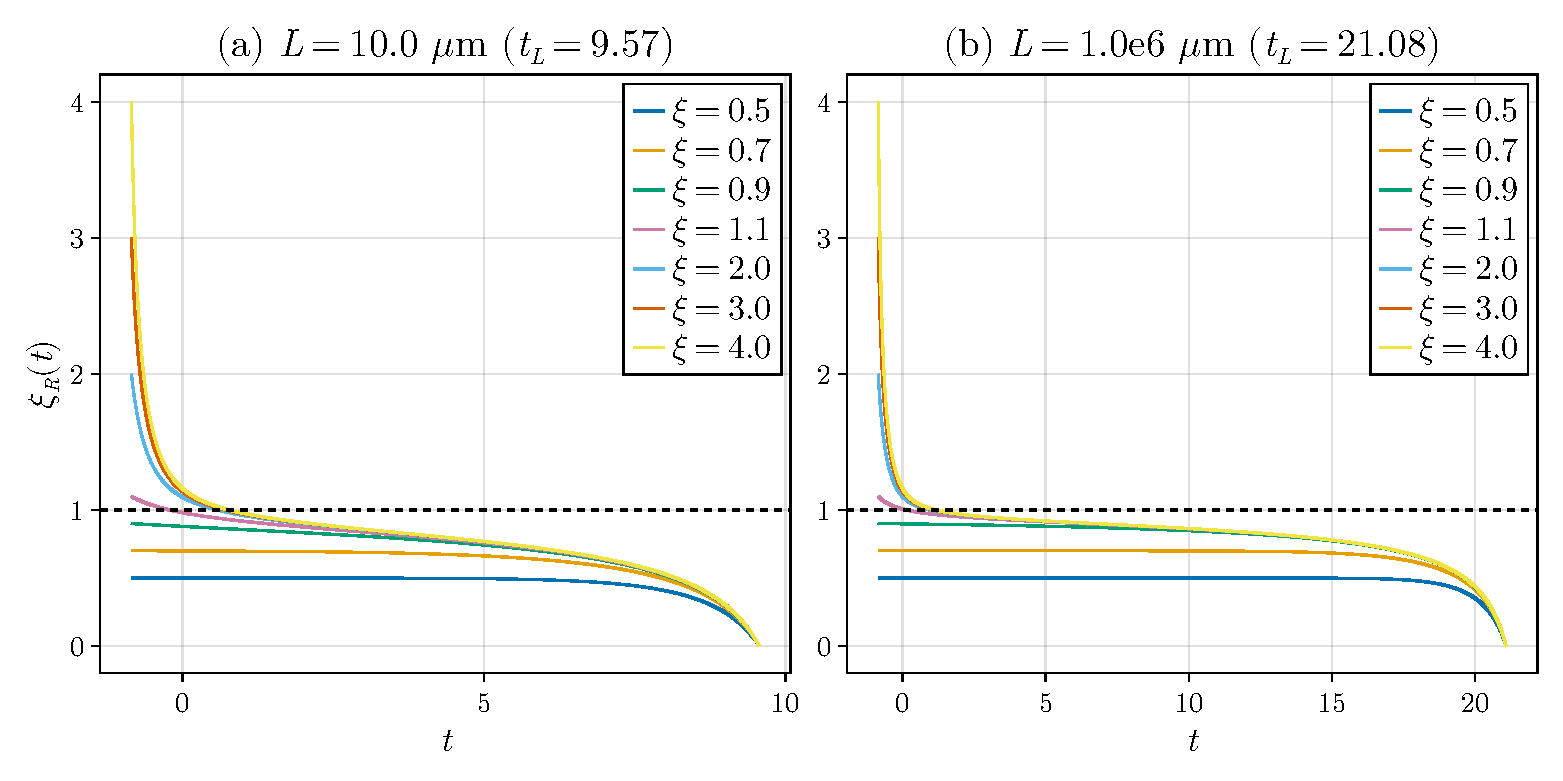
\includegraphics[width=0.9\textwidth]{./code/RG}
    \caption{RG方程式の数値解。パラメタは図\ref{fig:FKL}，\ref{fig:beta}と同じく$\ell_B=7$ \AA ，$a=3$ \AA ,そして，(a) $L=10 \mu$m，(b) $L=10^6 \mu$m とした。\label{fig:RG}}
  \end{center}
\end{figure}

一方で，$\xi>1$のときの$\xi_R$の減衰が，FKL厳密解と比較してRGの結果の方が急峻である。ただ，本稿でのRG解析はKatchalsky解の厳密な再現を目的とするものではなく，円筒PB方程式に現れる摂動項を再総和することで，くりこまれた線電荷のスケール依存性を抽出する近似的記述である。それにもかかわらず，$\xi>1$ での急速な$\xi_R\simeq 1$への接近，$\xi<1$での弱い流れ，セル境界近傍($t\simeq t_L$)での低下という本質的特徴はよく再現される。

\subsection{円筒形状(cylindrical geometry)の何が特別か -- RG解析による見方 --\label{sec:cylindrical_RG}}
\ref{sec:cylindrical}節では，平面や球と比較して円筒形状の何が特別かについてエネルギーとエントロピーの拮抗から議論した。ここでは平面と球の場合についても同様のRG解析を行うことで，円筒形状の特異性をRG解析の観点から理解することを試みる。結論から言うと，球や平面の場合には$\beta$関数の構造が円筒の場合とは大きく異なり，Manning-Oosawa凝集・非凝縮のような特徴的な振る舞いは現れないことになる。

数式をつかった詳しい議論を行う前に，$\beta$関数とRG flowの計算結果を見てみよう。図\ref{fig:RG_planar_spherical}には，平面と球の場合の$\beta$関数とRG方程式の数値解(RG flow)をプロットした。まず，(a)平面の場合の$\beta$関数は$\Sigma_R$の($\Sigma_R=0を除く$)全領域ではっきりと負である(図\ref{fig:RG_planar_spherical}(a-1))。したがって，$\Sigma_R$は$\ell$とともに減少し，固定点$\Sigma_R=0$に漸近する。特に，円筒の場合に見られたような$\xi_R$が1の近傍を通過する際に$\beta$が0に近づいていくような特徴的な振る舞いも見られない。$\beta$の$\ell$依存性はほとんどないが，$\ell$が境界値$\ell_L$に近づくと$\beta$が負に増大し，$\Sigma_R$がより速く(指数関数的に)0に近づいていくように働く。このような$\beta$関数の振る舞いは図\ref{fig:RG_planar_spherical}(a-2)に示したRG方程式の解に現れている。すなわち$\Sigma$の値によらずに$\Sigma_R$は$\ell$とともに減少し，$\Sigma_R$が特定の値の近傍を通過する際に$\beta$が0に近づいていくような特徴的な振る舞いも見られない。\textbf{つまり，$\Sigma_R$によらず，対イオンは平面に凝集し電荷のくりこみが起こることになる。これは電場のエネルギーが対イオンのエントロピーに対して常に支配的であるためである。}

\begin{figure}[htbp]
  \begin{center}
    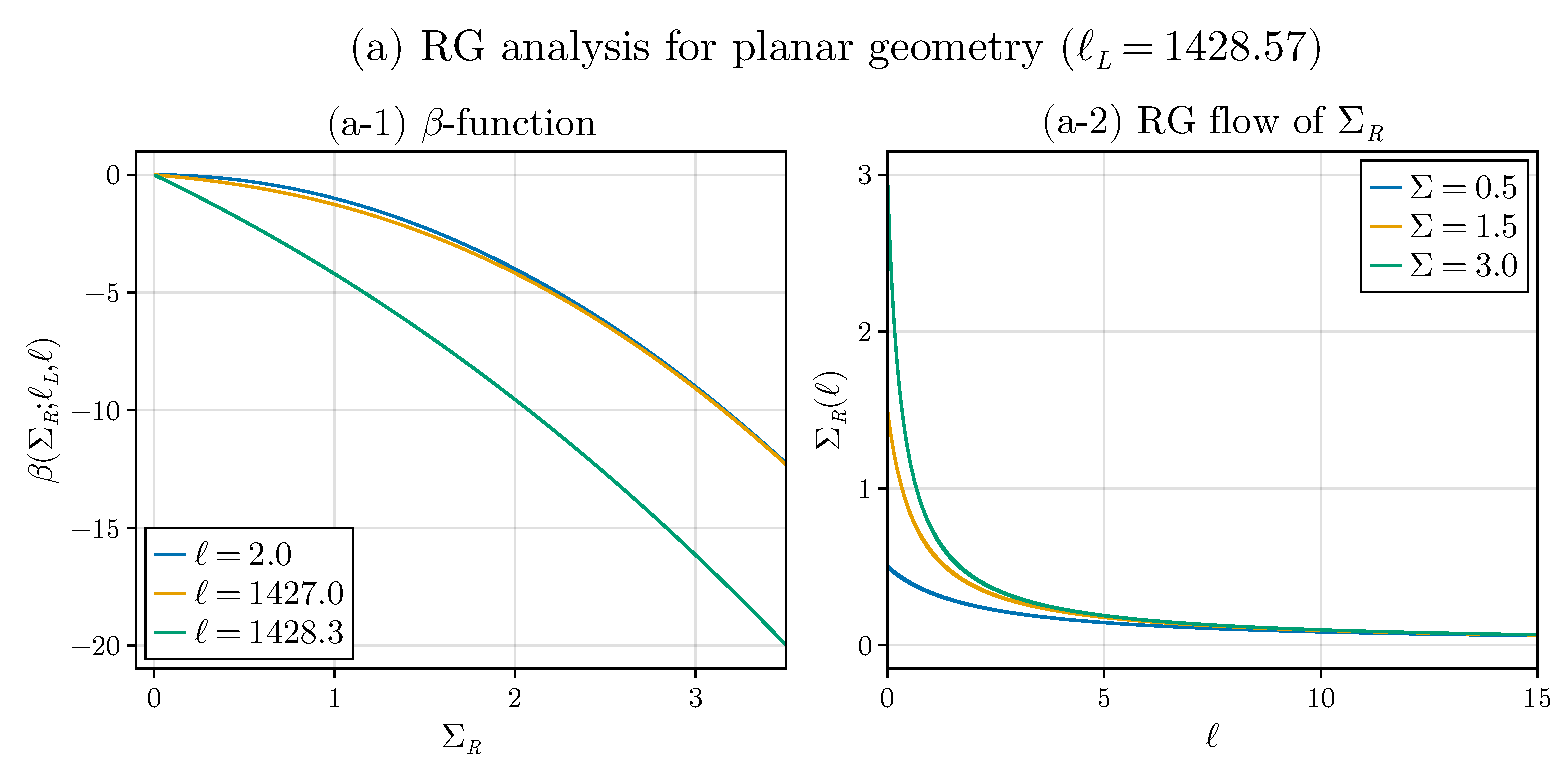
\includegraphics[width=0.9\textwidth]{./code/RG_planar}
    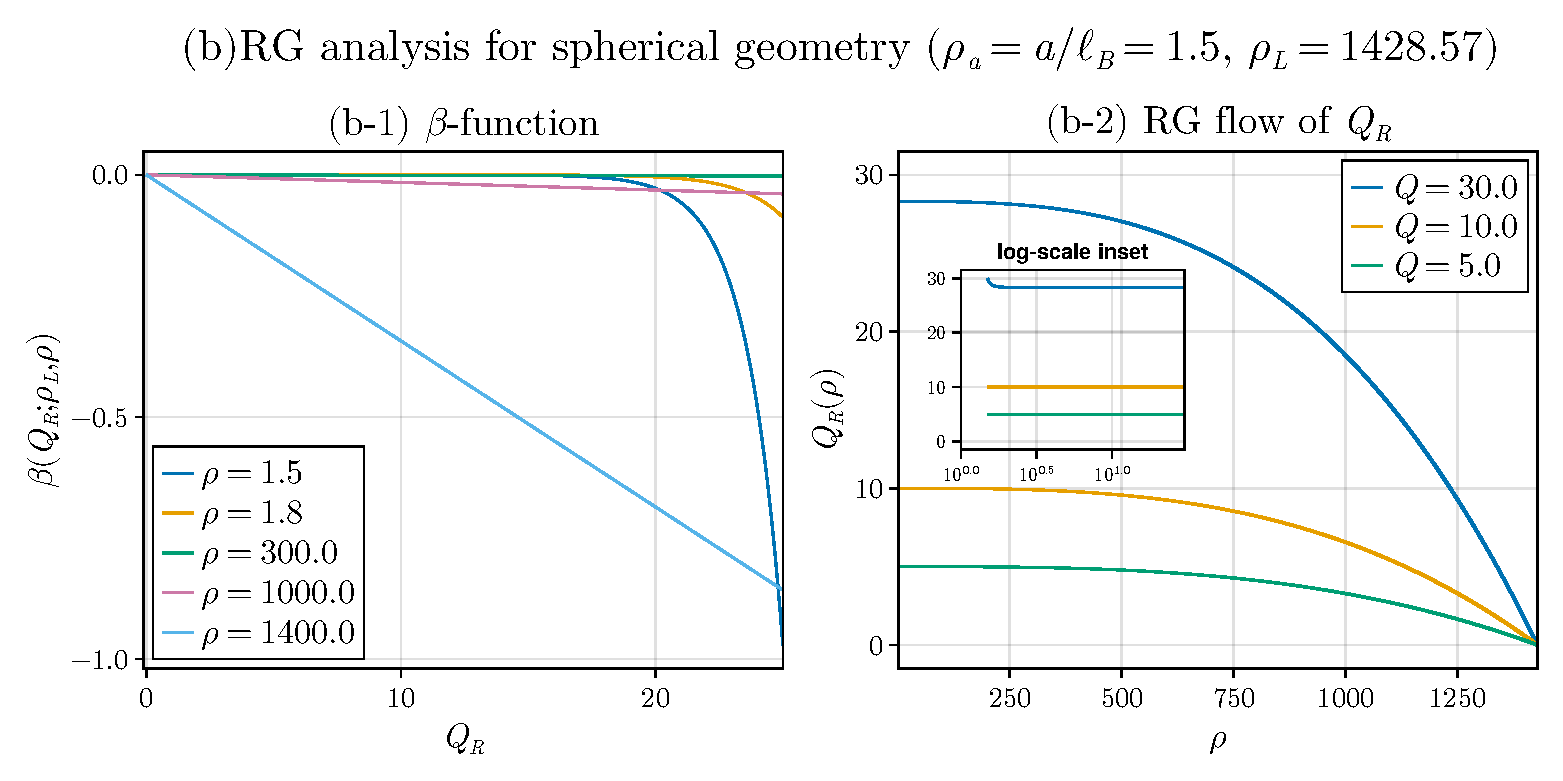
\includegraphics[width=0.9\textwidth]{./code/RG_spherical}
    \caption{(a)平面，(b)球の場合の$\beta$関数とRG方程式の数値解。パラメタは図\ref{fig:FKL}，\ref{fig:beta}, \ref{fig:RG}と同じく$\ell_B=7$とした。\label{fig:RG_planar_spherical}}
  \end{center}
\end{figure}

次に(b)球の場合を見てみよう。$\beta$関数の振る舞いは図\ref{fig:RG_planar_spherical}(b-1)に示した通りである。まず，$\rho$が小さいところ($\rho=$1.5, 1.8)では$\beta$は$Q_R$が小さいところではほぼゼロであるが，$Q_R$が大きいところでははっきりと負に増大している。$\rho$が大きくなるにつれて($\rho=300$, 1000)この傾向は無くなり$Q_R$の広い範囲で$\beta$はほぼゼロになる。すなわち$\rho$が小さなところでは僅かに電荷のくりこみがおこり$Q_R$は流れるが，その後，中間的な$\rho$では$Q_R$は殆ど流れない。$\rho$がさらに大きくなると$\beta$は全領域で負に増大していき，セル境界$\rho\to\rho_L$で，$Q_R\to 0$となる。このような$\beta$関数の振る舞いは図\ref{fig:RG_planar_spherical}(b-2)に示したRG方程式の解に現れている。図では$\rho_a$近傍での振る舞いが見やすいようにinsetで横軸を対数スケールにしたグラフも示している。$Q$が大きい時($Q=30$)には$\rho\simeq \rho_a$で僅かな減少が起こり$Q_R$が少し減少したあと，中間の$\rho$の範囲では$Q_R$はほとんど変化しない。さらに$\rho$が大きくなると，$\rho\to \rho_L$で境界条件に漸近($Q_R\to 0$)する。一方$Q$が小さいときには$\rho_a$近傍から中間領域まで$Q_R$は殆ど変化せず(流れず)に境界付近から境界条件に漸近する。

以上の結果を大まかにまとめると以下のようになる。平面の場合には$\Sigma_R$の値によらず$\beta$関数は有意に負であるから常に$\Sigma_R$は流れる。球の場合は$Q$が大きい場合には球近傍で$Q_R$は少し流れることもあるが，中間領域では$\beta$がほぼゼロになり$Q_R$は殆ど流れない。これらは，\textbf{やや乱暴に言えば，平面の場合は円筒の$\xi_R>1$のときのような振る舞い($\Sigma_R$を$\xi_R-1$に置き換えたような振る舞い)であり，球の場合は円筒の$\xi_R<1$のときのような振る舞いである。このことは，平面ではエネルギー優勢，球ではエントロピー優勢，円筒では両者が拮抗，という事実を反映している。} 表\ref{tab:geometry_RG}にはこのことを一覧にした。 以下ではここで述べたことを数式を使って詳しく議論する。



\begin{table}[t]
\centering
\caption{Comparison of RG flows for different geometries.}
\begin{tabular}{c|c|c|c|c}
\hline
Geometry & Coulomb potential & Entropy & RG behavior & Physical consequence \\
\hline
Plane &
$u(z)\sim z$ &
$\mathrm{const.}$ &
always flows &
always condensed
\\
Cylinder &
$u(r)\sim \log r$ &
$\log r$ &
marginal / nontrivial fixed point &
Manning condensation
\\
Sphere &
$u(r)\sim 1/r$ &
$\log r$ &
almost frozen &
almost diffuse
\\
\hline
\end{tabular}
\label{tab:geometry_RG}
\end{table}


\subsubsection{平面形状(plane geometry)}
まずは電荷密度$e\sigma(>0)$をもつ平面の場合を考える。平面の場合には，PB方程式は
\begin{align}
  \frac{d^2 u}{d\ell ^2} = - C e^{-u},\quad (\ell=z/\ell_B,\ C=4\pi\ell_B^3n_0) \label{eq:pb_plane}
\end{align}
となる。平面での電荷密度を$e\sigma$とすると，境界条件は
\begin{align}
  \left.\frac{du}{d\ell}\right|_{\ell=0} = 4\pi \ell_B^2 \sigma\equiv \Sigma, \quad \left.\frac{du}{d\ell}\right|_{\ell=\ell_L} = 0 \label{eq:boundary_plane}
\end{align}
である。平面の場合には，$\Sigma$が臨界値をまたいだときに解の振る舞いが大きく変わることはない。実際，円筒の時と同様に$\Sigma_R(\ell_R)$をパラメタとするPB方程式の解の族からRG方程式を構成すると，
\begin{align}
  \frac{d\Sigma_R}{d\ell} = \beta(\Sigma_R;\ell_L,\ell) \equiv -\frac{\Sigma_R^2}{1-e^{-\Sigma_R(\ell_L-\ell)}} \label{eq:beta_plane}
\end{align}
となる。円筒の場合と異なり，平面の場合は$\ell_L\to \infty$の極限が取れる。これは平面の場合は遠方でエントロピーと比較してエネルギーが支配的になってイオンが荷電平面に凝集しているからである。この極限では$\beta=-\Sigma_R^2$となり，$\Sigma_R$は$\ell$とともに減少していくことになる。\textbf{したがって，$\Sigma_R(0)=\Sigma$の値によらずくりこみ群の流れは固定点$\Sigma_R=0$に向かうことになる。つまり円筒の場合と異なり$\Sigma$が臨界値をまたいだときに解の振る舞いが大きく変わることはない。} ちなみに$\ell_L\to \infty$の極限，つまり$\beta=-\Sigma_R^2$のときはRG方程式は簡単に解けて$\Sigma_R(\ell)=1/(\Sigma^{-1}+ \ell)$である。じつは平面の場合のPB方程式は厳密解が知られており，$\Sigma_R=du/d\ell=2/[(\lambda_\mathrm{GC}/\ell_B)+\ell]=2/(2\Sigma^{-1}+\ell)$となる。ここで，$\lambda_\mathrm{GC}=1/(2\pi \ell_B^2 \sigma)=2\ell_B/\Sigma$はGouy-Chapman長である。したがって，RG方程式の解はPB方程式の1次近似解とはいえ，厳密解とかなり近い振る舞いをする。
\subsubsection{球形状(spherical geometry)}
次に球の場合を考える。$eQ(>0)$の電荷をもつ球の場合には，PB方程式は
\begin{align}
 \frac{1}{\rho^2}\frac{d}{d\rho}\left(\rho^2\frac{du}{d\rho}\right) = - C e^{-u},\quad (\rho=r/\ell_B,\ C=4\pi\ell_B^3n_0) \label{eq:pb_sphere}
\end{align}
境界条件は
\begin{align}
  \rho^2\left.\frac{du}{d\rho}\right|_{\rho=\rho_a} = Q, \quad \left.\frac{du}{d\rho}\right|_{\rho=\rho_L} = 0 \label{eq:boundary_sphere}
\end{align}
である。この場合もこれまでと同様にRG方程式を構成すると，
\begin{align}
  \frac{dQ_R}{d\rho} = \beta(Q_R;\rho_L,\rho) \equiv -\frac{\rho^2 Q_Re^{Q_R/\rho}}{I(Q_R;\rho_L,\rho)} \ (<0)\label{eq:beta_sphere}
\end{align}
となる。ただし
\begin{align}
  I(Q_R;\rho_L,\rho) = \int_\rho^{\rho_L}  s^2 e^{Q_R/s}  ds\label{eq:I_sphere}
\end{align}
である。ベータ関数の振る舞いを考察しよう。$\rho$が十分大きく$Q_R\ll\rho$の場合，式\eqref{eq:I_sphere}の非積分関数で$e^{Q_R/s}\simeq 1$と考えて良いので，$I\simeq (\rho_L^3-\rho^3)/3$となる。$I$は$\rho$の減少関数なので，全ての$\rho$に対して
\begin{align}
  I>(\rho_L^3-\rho^3)/3
\end{align}
である。したがって，
\begin{align}
  |\beta | < \frac{3\rho^2 Q_R e^{Q_R/\rho}}{\rho_L^3-\rho^3} \label{eq:beta_sphere_bound}
\end{align}
と上から抑えられる。すなわち，$\rho_L\to\infty$の極限では任意の有限な$Q_R$，$\rho$に対して$\beta\to 0$である。有限の$\rho_L$については，$e^{Q_R/\rho}/\rho_L \lesssim 1$であれば，あるいは$\rho$が大きくなって$Q_R$が少し``流れて''この不等式が満たされた段階では$|\beta|<3Q_R(\rho/\rho_L)^2/[1-(\rho/\rho_L)^3]$となる。したがって，$\rho$が$\rho_L$に近い場合を除けば$\beta$は非常に小さくなり，$Q_R$は$\rho$とともにほとんど変化せず，事実上$Q_R$は``流れない''。$\rho$が$\rho_L$に近い場合、$\beta$は非常に大きくなり、$Q_R$は急速に減少し，境界条件$Q_R(\rho_L)=0$を満たすようになる。

まとめると，\textbf{球では近距離で有限の charge renormalization が生じうるが，中間領域では $Q_R$ はほぼ一定となった後，セル境界$\rho\to\rho_L$で急激に$Q_R\to 0$となる。この中間領域での plateau は普遍的な値ではなく初期条件$Q$に依存するため，円筒におけるplateau，すなわち$\xi>1$ならば全て普遍的に$\xi_R=1$へ流れる場合とは異なる。}

%%%%%%%%%%%%%%%%% Salt effect %%%%%%%%%%%%%%%%%
\section{塩を加えた場合の荷電円筒 --MO普遍性の消失--}
ここまでは荷電高分子(円筒)の周りにその対イオンのみが存在する場合をあつかった。ここではそこにさらに塩(正・負イオン)を添加した場合を考える。この場合はPB方程式は\eqref{eq:pb}から変更を受けて，
\begin{align}
  \frac{1}{r}\frac{\dd}{\dd r}\left(r\frac{\dd u}{\dd r}\right)=-4\pi \ell_Bn_0 (e^{-u}-e^{u}), \label{eq:pb_salt}
\end{align}
となる。あるいは対数座標$t=\log(r/\ell_B)$では\eqref{eq:pb_t}から
\begin{align}
  \frac{d^2 u}{dt^2} = -4\pi n_0\ell_B^3 (e^{-u+2t}-e^{u+2t}) \label{eq:pb_salt_t}
\end{align}
となる。右辺のカッコ内第1項が正のイオン，第2項が負のイオンに対応する。無限系で十分遠方では電気的中性が成り立つのでカッコ内はゼロ，すなわち$u=0$となる。したがって$n_0$は無限遠での塩濃度である。境界条件は式\eqref{eq:boundary_t}と同じである。

円筒近傍では電場が強く，一般には$|u|$は大きいが，十分遠方では$|u|\ll 1$となり，そこでは式\eqref{eq:pb_salt}右辺は$u$に関して線形化できるであろう。すると，線形化PB方程式 (LPB)
\begin{align}
  \frac{1}{r}\frac{\dd}{\dd r}\left(r\frac{\dd u}{\dd r}\right)=\kappa^2 u \label{eq:lpb}
\end{align}
が得られる。ここで，
\begin{align}
  \kappa=\sqrt{8\pi\ell_B n_0}
\end{align}
はDebye波数で，その逆数$\kappa^{-1}$はDebye長と呼ばれる。その対数を
\begin{align}
  \tD\equiv \log(\kappa^{-1}/\ell_B)
\end{align}
と定義しておく。大まかにいえば，遠方では$u$は$e^{-\kappa r}$で減衰する。

\textbf{一般に，$r\lesssim \kappa^{-1}$ (対数座標では$t\lesssim \tD$)では円筒による電場が強く非線形性が無視できないが，$r\gtrsim \kappa^{-1}$ ($t\gtrsim \tD$)では十分に対イオンによる遮蔽が起こり線形化PBが使える。}まずはこのことを実際に確認しよう。式\eqref{eq:pb_salt}は一般には厳密解は知られていないので数値的に解いたものを図\ref{fig:PBsalt_sim}にプロットした(塩なしの場合との比較がしやすいように$u$ではなく$\xi_R(t)=(1/2)(du/dt)$をプロットしている)。2本の曲線はそれぞれ低塩濃度($\tD=7.6$)と高塩濃度($\tD=1.84$)に対応する。どちらも$t$が$\tD$を超えると速やかに減衰しゼロになっている。

\begin{figure}[htbp]
  \begin{center}
    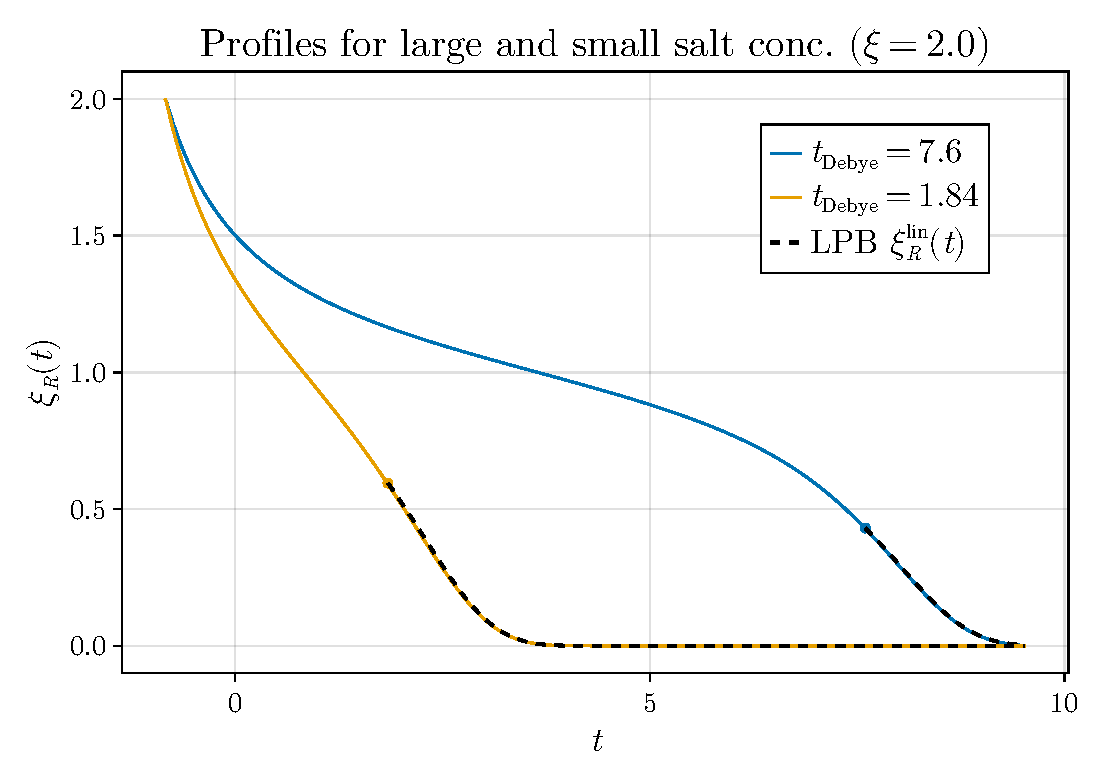
\includegraphics[width=0.7\textwidth]{./code/simulation/profile_salt_LPB}
    \caption{塩ありPBの数値解。遠方($t>\tD$)では線形化PBの解を破線でプロットした。\label{fig:PBsalt_sim}}
  \end{center}
\end{figure}

ここで，中心からデバイ長の場所$r=\kappa^{-1}$でのrenormalized chargeを\textbf{塩系における有効電荷}$\xi_\mathrm{eff}$と定義する:
\begin{align}
  \xi_\mathrm{eff}=\xi_R(\tD).
\end{align}
この場所$t=\tD$で境界条件$\xi_R^\mathrm{lin}(\tD)=\xi_\mathrm{eff}$を与えた場合の線形化PB\eqref{eq:lpb}は厳密に解けて，
\begin{align}
  \xi_R^\mathrm{lin}(t)=\frac{\xi_\mathrm{eff}}{K_1(1)}\kappa r K_1(\kappa r)=\frac{\xi_\mathrm{eff}}{K_1(1)}e^{t-\tD}K_1(e^{t-\tD})
\end{align}
となる。ここで$K_\nu$は第二種変形Bessel関数である。図\ref{fig:PBsalt_sim}にはこの線形PBの解もそれぞれの塩濃度に対して破線でプロットしてある。(非線形)PBの解とよく一致していることがわかる。



\subsection{有効電荷$\xi_\mathrm{eff}=\xi_R(\tD)$のManning パラメタ・塩濃度依存性(数値解) \label{sec:xieff}}
Manning-Oosawa凝集と結びつけるために，有効電荷$\xi_\mathrm{eff}=\xi_R(\tD)$のManning パラメタ・塩濃度依存性を議論する。図\ref{fig:xieff}には４つの塩濃度(対応する$\tD$は塩濃度が小さいほうから7.6, 5.3, 2.99, 1.84)に対して，Manningパラメタ$\xi$の関数として有効電荷$\xi_\mathrm{eff}$をプロットした。

\begin{figure}[htbp]
  \begin{center}
    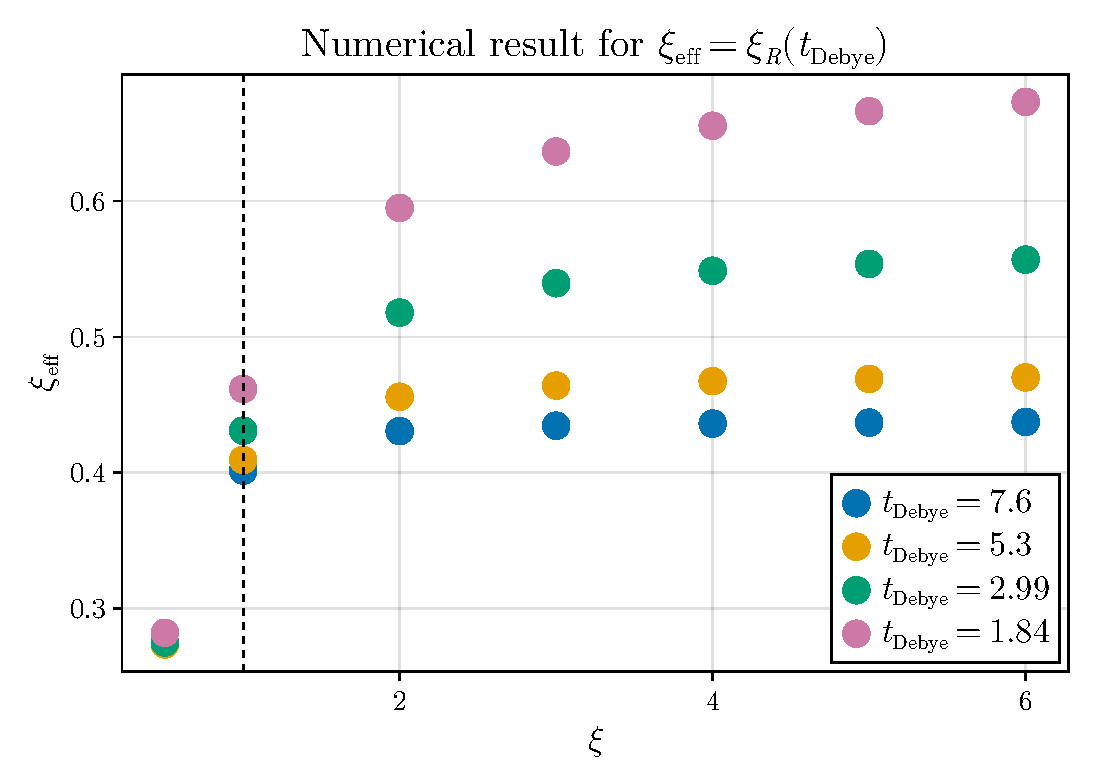
\includegraphics[width=0.7\textwidth]{./code/simulation/xi_eff}
    \caption{PBの数値解から求めた有効電荷$\xi_\mathrm{eff}=\xi_R(\tD)$のManning パラメタ・塩濃度依存性。\label{fig:xieff}}
  \end{center}
\end{figure}

いずれの塩濃度でも$\xi$が大きくなるにつれて$\xi_\mathrm{eff}$が増大するが，塩濃度が小さい場合($\tD=7.6$, 5.3)では$\xi$が1を超えるとほぼ平坦，すなわち$t\gtrsim \tD$ ($r\gtrsim \kappa^{-1}$)では$\xi>1$のManningパラメタの円筒は同一に見える，というManning-Oosawa凝集の特徴が保持されている。しかし塩濃度が大きくなるにつれ($\tD=2.99$, 1.84)，$\xi$が1を超えても$\xi_\mathrm{eff}$の増大が止まらなくなる。このように，\textbf{塩濃度が大きくなるにつれてManning-Oosawa凝集の普遍性が消失する。}

このことを直観的に理解しやすくするために図\ref{fig:profile_salt}に(a)低塩濃度($\tD =7.6$)および(b)高塩濃度($\tD=0.69$)におけるPB方程式の数値解を示した。それぞれ5つのManningパラメタ$\xi$に対する解をプロットしてある。縦破線は$t=\tD$を示し，この線を横切る時の$\xi_R$が$\xi_\mathrm{eff}$に対応している。この図では，塩濃度が小さいときは$\tD$が大きく,
$\xi>1$の解が$t$がある程度大きいところではほぼ同一曲線に乗る。一方，塩濃度が大きくなると$\tD$が小さくなるために，異なる$\xi$に対応する$\xi_R(t)$曲線が``重なる前に''$t$が$\tD$に達してしまい，そのまま$\xi_R$は減衰してしまっているように見える。

\begin{figure}[htbp]
  \begin{center}
    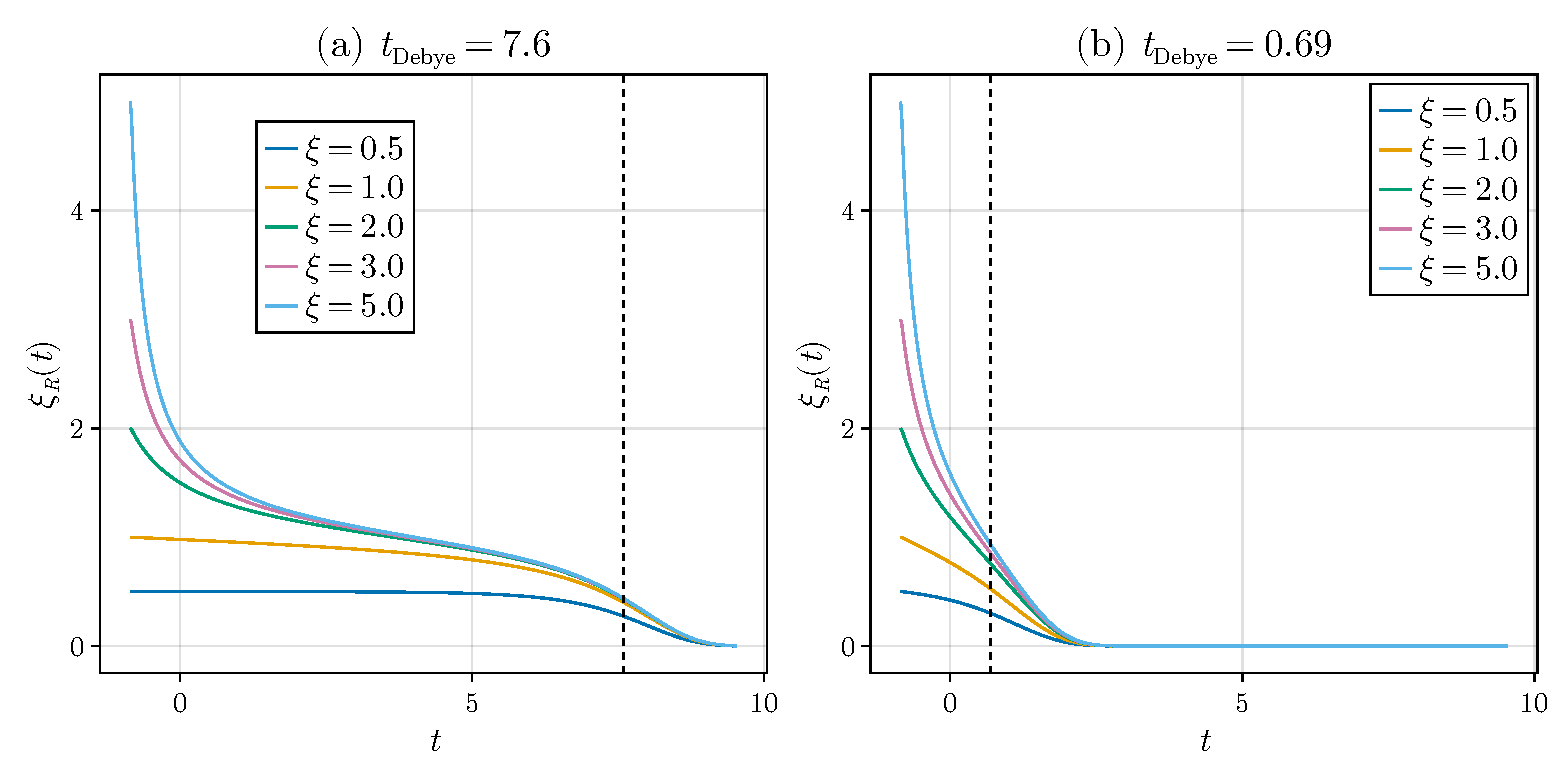
\includegraphics[width=0.9\textwidth]{./code/simulation/profile_salt}
    \caption{(a)低塩濃度($\tD =7.6$)および(b)高塩濃度($\tD=0.69$)における数値解。破線は$t=\tD$を示し，ここを横切る際の$\xi_R$が$\xi_\mathrm{eff}$に対応する。\label{fig:profile_salt}}
  \end{center}
\end{figure}


このことを理解するためには次のような考え方が有効である。$r\lesssim \kappa^{-1}$では円筒の電場が強く$|u|\gtrsim 1$であるため，共イオン(円筒と同符号の電荷をもつイオン)は遠くにはじかれてしまってほぼ存在せず，塩なしのPBが使える。このことは図\ref{fig:profile_salt}(a)の$t\lesssim \tD$の振る舞いが図\ref{fig:FKL}の解曲線と酷似していることからも納得されるだろう。すなわち以下の描像が成り立つであろう:
\begin{pointbox}[title=重要(塩ありPB解の振る舞い)]
荷電円筒の十分遠く($r\gtrsim \kappa^{-1}$)では，$r=\kappa^{-1}$における有効電荷$\xi_\mathrm{eff}=\xi_R(\kappa^{-1})$を境界条件とした線形化PBの解に従う。一方，荷電円筒の近く($r\lesssim \kappa^{-1}$)では電場が強く，共イオンはほとんど存在できないため，塩なしPB方程式の解で近似できる。

もちろん実際には，これら二つの領域は$r\sim \kappa^{-1}$付近でなめらかにつながっており，厳密な境界があるわけではない。しかし本質的な物理を理解するには，上記のように二つの領域に分けて考えると非常にわかりやすい。
\end{pointbox}



このような考え方に立てば，$r<\kappa^{-1}$の領域に塩なしの場合のRG解析の考えを適用して，次のようにして塩添加効果を理解できるであろう。すなわち，塩が希薄な場合には，$\kappa^{-1}$ (あるいは$\tD$)が大きいため，RG flowが十分``長時間''流れて，$\xi>1$の解曲線群が$\xi_R\simeq 1$の普遍的 plateau に達してManning-Oosawa凝集が保持される。一方，塩が濃厚になると，$\kappa^{-1}$ ($\tD$)が小さくなり，RG flowが十分流れず，$\xi>1$の解曲線群が$\xi_R=1$にまで到達できない。\textbf{すなわち，$\tD$がRGの赤外カットオフとして作用し，その大小によって普遍的plateau $\xi_R\simeq 1$にまで到達できるか否かが，Manning–Oosawa 凝集が観測されるか否かを決定する，という構造である}。

\subsection{RG解析 --塩効果から生じる赤外カットオフによるMO普遍性の消失--}
直前の\ref{sec:xieff}節最後に書いた考え方に基づいて具体的にRG flowを計算する。やることは，RG方程式 \eqref{eq:beta_function}を初期値を$\xi_R(t_a)=\xi$として$t=\tD$まで積分するだけである。ここでは簡単のため，$L\to\infty$として，
\begin{align}
  \frac{d\xi_R}{dt}=\begin{cases}
0   & (\xi_R<1) \\
-2\xi_R(\xi_R-1)  & (\xi_R>1)
\end{cases} \label{eq:RG_infinite}
\end{align}
を使う。丁寧にやるなら，有限セルで外側境界条件に$\xi_R(t_L)=\xi_\mathrm{eff}$を課して，外側の線形PB解とつなぐ，ということになるであろうが，ここでの目的は精密に厳密解に近づけることではないので，簡便法で進める。式\eqref{eq:RG_infinite}は分離系なので解析的に解けて，
\begin{align}
  \xi_R(t)=\begin{cases}
\xi & (\xi<1)  \\
\frac{\xi}{\xi-(\xi-1)e^{-2(t-t_a)}} & (\xi>1)
\end{cases}
\end{align}
となる。すなわち，$\xi<1$であれば凍結され，$\xi>1$ならば，$t$が大きくなるにつれて
$\xi_R(t)\sim 1+(\xi-1)\xi^{-1}e^{-2(t-t_a)}$となり，指数的に1に近づく。$\xi>1$であっても，塩添加により生じる赤外カットオフ$\tD$が小さければこのflowは普遍的 plateau に到達する前に打ち切られる。結果を図\ref{fig:RG_salt}に示した。ここまでの議論で予想したとおりの結果となっている。図\ref{fig:xieff}に示した数値計算の結果と比較すれば定量的一致は無いが，それでも(かなりの近似計算にも関わらず)定性的特徴はよく捉えている。

\begin{figure}[htbp]
  \begin{center}
    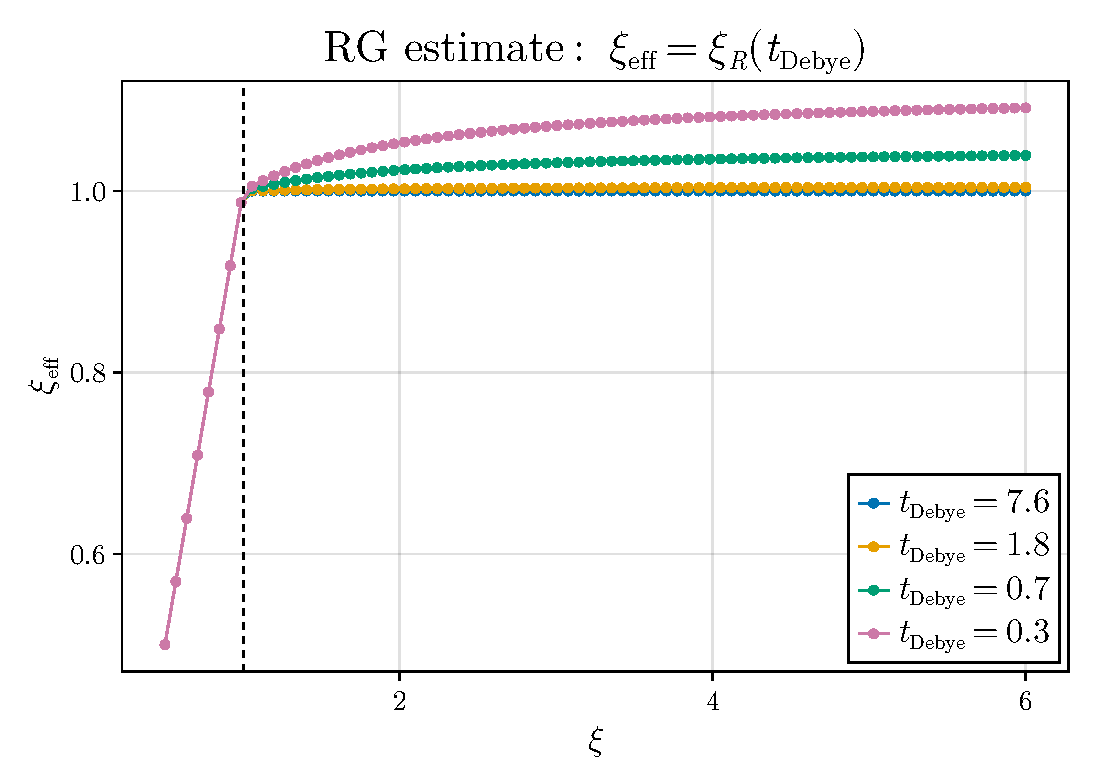
\includegraphics[width=0.7\textwidth]{./code/xi_eff_RG_salt_cutoff}
    \caption{RG方程式による$\xi_\mathrm{eff}$の見積もり。\label{fig:RG_salt}}
  \end{center}
\end{figure}
%%%%%%%%%%%%%%%%% APPENDIX %%%%%%%%%%%%%%%%%

\appendix
\newpage
\section{FKL厳密解の詳細\label{appendix:FKL}}
元の式の無次元化ポテンシャル$u$を
\begin{equation}
u(r)=2t+w(t)
\end{equation}
と変数変換すると，PB方程式は
\begin{equation}
\frac{d^2 w}{dt^2}
=-C e^{-w}
\label{Liouville_form}
\end{equation}
という Liouville 型方程式へ変換される。
ここで
\(C\)
は定数である。
この式は1次元力学系に類似した構造を持つ。
実際，1回積分すると
\begin{equation}
\left(\frac{dw}{dt}\right)^2
=4(A-Ce^{-w})
\label{first_integral}
\end{equation}
となる。
ここで
\(A\)
は積分定数である。
重要なのは，この積分定数
\(A\)
の符号によって解の構造が分岐することである。


\subsection{Trigonometric branch}

まず
\begin{equation}
A>0
\end{equation}
の場合を考える。
このとき解は三角関数型となり，
\begin{equation}
u(t)
=
2(t-t_L)
+
2\log
\left[
\frac{
\cos\{\gamma(t-t_M)\}
}{
\cos\{\gamma(t_L-t_M)\}
}
\right]
\label{trig_solution}
\end{equation}
と書ける。
ここで
\begin{equation}
t_L=\log(L/\ell_B)
\end{equation}
であり，
\(L\)
はセル半径である。
また
\(\gamma\)
および
\(t_M\)
は境界条件から決まる定数である。
有効 Manning parameter を
\begin{equation}
\xi_R(t)
\equiv
\frac12\frac{du}{dt}
\label{xiR_def}
\end{equation}
と定義すると，
\begin{equation}
\xi_R(t)
=
1-\gamma \tan\{\gamma(t-t_M)\}
\label{xiR_trig}
\end{equation}
となる。
境界条件
\begin{equation}
\xi_R(t_L)=0
\end{equation}
より
\begin{equation}
\tan\{\gamma(t_L-t_M)\}
=\frac1\gamma
\label{boundary_trig_1}
\end{equation}
が得られる。
さらに円筒表面
\(r=a\)
における条件
\begin{equation}
\xi_R(t_a)=\xi
\end{equation}
を用いると，
\begin{equation}
\tan\{\gamma(t_a-t_M)\}
=\frac{1-\xi}{\gamma}
\label{boundary_trig_2}
\end{equation}
となる。
これらを組み合わせると，
\begin{equation}
\gamma \log\frac{L}{a}
=
\tan^{-1}\frac1\gamma
-
\tan^{-1}\frac{1-\xi}{\gamma}
\label{gamma_equation}
\end{equation}
が得られる。
この branch は，有限セル系では
\begin{equation}
\xi>\xi_c
\end{equation}
で存在する。
ここで
\begin{equation}
\xi_c
=
\frac{\log(L/a)}{1+\log(L/a)}
\label{xi_c}
\end{equation}
である。
特に
\(L/a\to\infty\)
では
\begin{equation}
\xi_c\to1
\end{equation}
となり，Manning-Oosawa の閾値
\(\xi=1\)
が現れる。


\subsection{Hyperbolic branch}

次に
\begin{equation}
A<0
\end{equation}
の場合を考える。
このとき解は双曲線関数型となり，
\begin{equation}
u(t)
=
2(t-t_L)
+
2\log
\left[
\frac{
\sinh\{\alpha(t_0-t)\}
}{
\sinh\{\alpha(t_0-t_L)\}
}
\right]
\label{hyperbolic_solution}
\end{equation}
と書ける。
有効 Manning parameter は
\begin{equation}
\xi_R(t)
=
1-\alpha\coth\{\alpha(t_0-t)\}
\label{xiR_hyper}
\end{equation}
となる。
境界条件より
\begin{equation}
\coth\{\alpha(t_0-t_L)\}
=\frac1\alpha
\label{boundary_hyper_1}
\end{equation}
および
\begin{equation}
\coth\{\alpha(t_0-t_a)\}
=\frac{1-\xi}{\alpha}
\label{boundary_hyper_2}
\end{equation}
が得られる。
したがって
\begin{equation}
\alpha \log\frac{L}{a}
=
\tanh^{-1}\alpha
-
\tanh^{-1}\frac{\alpha}{1-\xi}
\label{alpha_equation}
\end{equation}
となる。
この branch は
\begin{equation}
\xi<\xi_c
\end{equation}
で存在する。


\subsection{臨界 branch}

境界
\begin{equation}
\xi=\xi_c
\end{equation}
では
\begin{equation}
\gamma\to0,
\qquad
\alpha\to0
\end{equation}
となり，解は有理関数型へ移行する。
このとき
\begin{equation}
u(t)
=
2(t-t_L)
+
2\log
\left[
\frac{t_0-t}{t_0-t_L}
\right]
\label{critical_solution}
\end{equation}
となる。
対応する有効 Manning parameter は
\begin{equation}
\xi_R(t)
=
1-\frac1{t_0-t}
\label{critical_xiR}
\end{equation}
である。


\subsection{Manning凝集との関係}

Trigonometric branch では，
\begin{equation}
\xi_R(t)\simeq1
\end{equation}
となる広い領域が現れる。
これは Manning-Oosawa 対イオン凝集に対応する。
すなわち，裸の Manning parameter が
\begin{equation}
\xi>1
\end{equation}
であっても，遠方から見た有効電荷は
\begin{equation}
\xi_R\simeq1
\end{equation}
へ renormalize される。
一方，
\(\xi<1\)
ではそのような plateau は現れず，
有効電荷は裸電荷に近い値を保つ。
有限セルでは branch point は
\(\xi_c<1\)
へずれるが，
無限希釈極限
\(L/a\to\infty\)
では
\(\xi_c\to1\)
となる。
したがって Manning-Oosawa 対イオン凝集は，
円筒 geometry に由来する logarithmic interaction によって生じる，臨界的な charge renormalization と理解できる。

\printbibliography


\end{document}